
We consider PDE examples with repeated parametric and sector-bounded
uncertainties. For additional information on the problem setup, the reader is
referred to \url{https://github.com/TMLenssen/PIETOOLS-Duality}.

\subsection{Note on loop shifting with $\mcl J$}

In our examples we perform the loop shift $\frac{\partial}{\partial s}
\circ\Delta$ on distributed uncertainty channels entering the dynamics.
The effect of this loop shift can be seen from
$\dot{\mbf v}=\mbf v_{ss}+\delta^2\mbf v$, with $\mbf v(t,0)=0$ and
$|\delta|\leq\alpha$. Representing $\delta^2$ by two repeated channels and
spatially differentiating their inputs and outputs gives
\begin{align*}
 \dot{\mbf v}&=\mbf v_{ss}+\mcl Jw_{\Delta,2},\\
 z_{\Delta,1}&=\mbf v_s,\qquad z_{\Delta,2}=w_{\Delta,1},\\
 w_{\Delta,i}&=\delta z_{\Delta,i},\qquad i\in\{1,2\}.
\end{align*}
Define the spatial integration operator $\mcl J\in\Pi_3$ by
$(\mcl Jf)(t,s):=\int_0^s f(t,\theta)\,d\theta$.
Closing the loop recovers
$\mcl Jw_{\Delta,2}=\delta^2\mcl J\mbf v_s=\delta^2\mbf v$. The
feedthrough $z_{\Delta,2}=w_{\Delta,1}$ remains unfiltered, since filtering
it would instead produce the different term $\delta^2\mcl J\mbf v$. This
realization substantially improves feasibility in our computations,
possibly because it better aligns with the fundamental PIE state. We do not
have a general analytical explanation and therefore treat this benefit as
empirical and realization- and uncertainty-dependent.

\subsection{Primal--dual analysis with repeated real uncertainty}
\label{ex:coupled-heat}


\begin{figure*}[t]
 \centering
 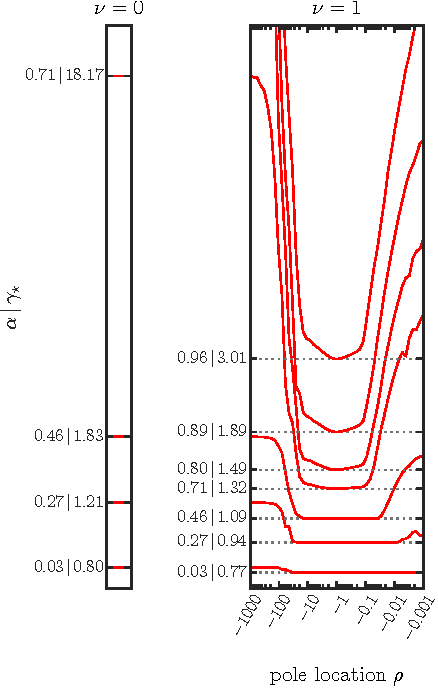
\includegraphics[height=.52\textwidth]{Figures/example1_primal.pdf}\hfill
 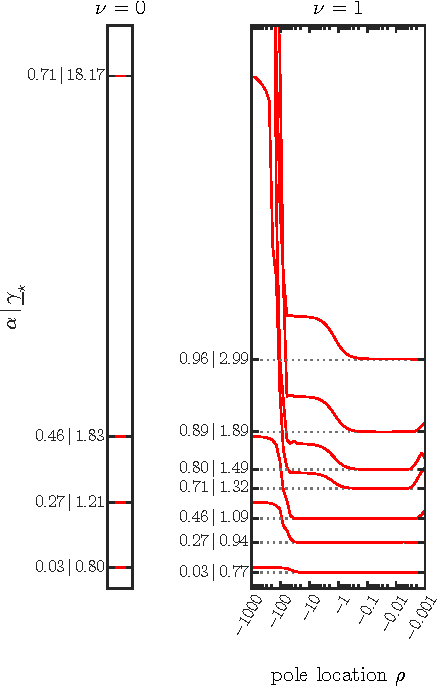
\includegraphics[height=.52\textwidth]{Figures/example1_dual.pdf}\hfill
 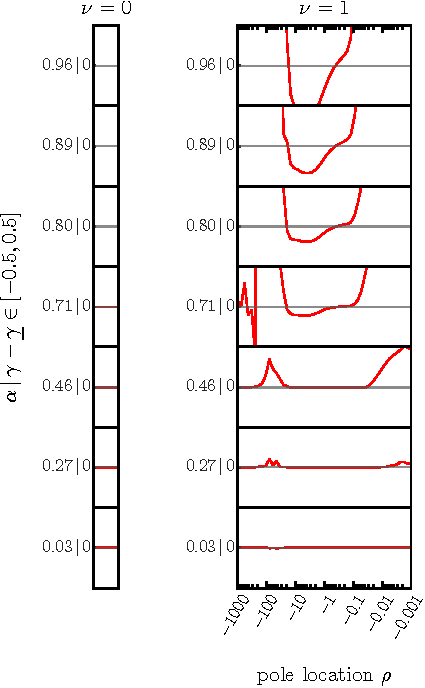
\includegraphics[height=.52\textwidth]{Figures/example1_difference.pdf}
 \caption{Reproduction of the sweep in \cite[Fig.~7]{veenman2016robust} for the coupled heat equations:
  primal analysis (left), dual analysis (center), and the difference $\gamma-\underline{\gamma}$ 
  between the primal and dual bounds (right). The figure highlights two main observations. First, 
  even when using a lifted finite-dimensional filter for the dynamic IQC, the choice $\nu=1$ yields 
  substantially smaller values of $\gamma$ than the static case $\nu=0$. Second, the dual analysis 
  produces lower values of $\gamma$ than the primal analysis. This indicates that, for the chosen IQC 
  parameterization, the dual formulation yields less conservative bounds and allows the small-gain 
  bound on $G_0$ to be pushed closer to $\rho=1$. This difference is possible because the problem is 
  formulated such that $\Theta$ need not coincide with $\mbf{D}(\Theta)$, so the primal and dual 
  analyses need not yield identical bounds under the same lifted finite-dimensional filter 
  parameterization, which may be better suited to the dual system than to the primal system.
}
\label{fig:coupled-heat-primal-dual}
\end{figure*}%
We begin with the finite-dimensional ODE benchmark
in~\cite[Sec.~8.1]{veenman2016robust}. We copy its temporal filter basis, 
and performance setup, and apply the same
construction to a pair of coupled heat equations by lifting the filter over the 
spatial domain. For the static part we can use general PI operators. This multiplier
setup aligns with the multiplier class in \cite[Lem.~10]{10156335}. We use
the same finite-dimensional matrices, with some
perturbation on $A$, as in the ODE benchmark, but apply them on
distributed signals, and add a diffusion
term to obtain the coupled PDE. Let $s\in[0,1]$ and
\begin{align*}
 A&=\bmat{-2&-3\\1&1}+\frac{\pi^2}{2}I,
 &B_\Delta&=\bmat{1&0\\0&0},&B_{\mrm p}&=\bmat{1\\0},\\
 C_\Delta&=\bmat{1&0\\0&0},
 &D_{\Delta}&=\bmat{1&-2\\1&-1},
 &D_{\Delta\mrm p}&=\bmat{0\\1},\\
 C_{\mrm p}&=\bmat{1&0},
 &D_{\mrm p\Delta}&=\bmat{0&1}.
\end{align*}
Consider
\begin{align*}
 \dot{\mbf v}&=\mbf v_{ss}+A\mbf v
      +B_\Delta\mcl Jw_\Delta+sB_{\mrm p}w_{\mrm p},\\
 z_\Delta&=C_\Delta\mbf v_s+D_{\Delta}w_\Delta
      +D_{\Delta\mrm p}w_{\mrm p},\\
 z_{\mrm p}&=\int_0^1\left(C_{\mrm p}\mbf v
      +2D_{\mrm p\Delta}\mcl Jw_\Delta\right)ds,\\
      \mbf v(t,0)&=0,\quad \mbf v_s(t,1)=0,\\
      w_\Delta&=\delta z_\Delta,\quad |\delta|\leq\alpha,\\
\end{align*}
We convert this system to a PIE using the PIETOOLS toolbox
\cite{pietools2025manual}. We find that the uncertainty-channel
PIE feedthrough $\mcl D_\Delta: w_\Delta \to z_\Delta$ acts pointwise:
\begin{align*}
 (\mcl D_\Delta\mbf q)(t,s)&=D_\Delta\mbf q(t,s),\\
 (\mcl D_\Delta\Delta\mbf q)(t,s)&=\delta D_\Delta\mbf q(t,s).
\end{align*}
Consequently, the algebraic well-posedness condition reduces to
\begin{equation*}
 \det(I_2-\delta D_\Delta)
 =\det\bmat{1-\delta&2\delta\\-\delta&1+\delta}
 =1+\delta^2>0.
\end{equation*}
Hence $I-\mcl D_\Delta\Delta$ has a bounded inverse for
every real $\delta$.
The same real
scalar $\delta$ is repeated over both channels and all spatial
locations, and $\Delta=\delta I$ is self-adjoint, bounded, time-invariant and memoryless. 
We therefore use the same
multiplier family in the two analyses,
\begin{align*}
 &\mcl V_\Delta\{\alpha^2\mcl Q_\Delta,
 \alpha\mcl S_\Delta,-\mcl Q_\Delta\},\quad
 \mcl Q_\Delta\succeq0\in\Pi_4,\quad \mcl S_\Delta^*=-\mcl S_\Delta\in\Pi_4, \\
&\underline{\mcl V}_\Delta\{\alpha^2\underline{\mcl Q}_\Delta,
 \alpha\underline{\mcl S}_\Delta,-\underline{\mcl Q}_\Delta\},\quad
 \underline{\mcl Q}_\Delta\succeq0\in\Pi_4,\quad \underline{\mcl S}_\Delta^*=-\underline{\mcl S}_\Delta\in\Pi_4.
\end{align*}
This is the situation
described in Section~\ref{sec:dynamic-filtering-duality-1}, because
$\Delta=\Delta^*$, the primal and dual certificates can use the same dynamic
filter and repeated-real IQC structure \cite[Lem.~10]{10156335}. The dynamic uncertainty filter is constructed from the stable temporal
basis~\cite[Eq.~(12a)]{veenman2016robust},
\begin{equation*}
 \psi_\nu(i\omega)=\bmat{1&\dfrac{1}{i\omega-\rho}&\cdots&
 \dfrac{1}{(i\omega-\rho)^\nu}}^{\!T},
 \qquad \rho<0,
\end{equation*}
For $\nu\geq1$, define the finite-dimensional realization
\begin{align*}
 A_\nu&=\bmat{
  \rho&0&\cdots&0\\
  1&\rho&\ddots&\vdots\\
  0&\ddots&\ddots&0\\
  0&\cdots&1&\rho}\in\R^{\nu\times\nu},
 &B_\nu&=\bmat{1\\0\\\vdots\\0}\in\R^{\nu\times 1},\\
 C_\nu&=\bmat{0_{1\times\nu}\\I_\nu}\in\R^{1+\nu\times\nu},
 &D_\nu&=\bmat{1\\0_{\nu\times1}}\in\R^{1+\nu\times 1}.
\end{align*}
Since there are two uncertainty channels,
define the PI operators pointwise by
\begin{align*}
 (\mcl T\mbf q)(s)&=\mbf q(s),&\\
 (\mcl A\mbf q)(s)&=(A_\nu\otimes I_2)\mbf q(s),&(\mcl B\mbf{q})(s)&=(B_\nu\otimes I_2)\mbf q(s),\\
 (\mcl C\mbf q)(s)&=(C_\nu\otimes I_2)\mbf q(s),&(\mcl D\mbf{q})(s)&=(D_\nu\otimes I_2)\mbf{q}(s).
\end{align*}
Thus the lifted basis function satisfies ${\psi}\{\mcl T,\mcl A,\mcl B,\mcl C,\mcl D\}$.  The uncertainty filter
used in both analyses is
\begin{equation}\label{eq:example-shared-filter}
 \underline{\Psi}_\Delta=\Psi_\Delta
 :=\bmat{\psi&0\\0&\psi},\qquad \Psi_\Delta\bmat{z_\Delta\\w_\Delta}.
\end{equation}
In particular, no distinct dual filter is introduced in this example. The
gain from $w_{\mrm p}$
to $z_{\mrm p}$ is tested with the induced $L_2$-gain performance multipliers
$\mcl V_{\mrm p}\{1,0,-\gamma^2\}$ and
$\underline{\mcl V}_{\mrm p}\{1,0,-\underline\gamma^2\}$, respectively.
Table~\ref{tab:coupled-heat-timing} shows that computation time increases
sharply with filter order.
We therefore perform the full pole sweep in
Figure~\ref{fig:coupled-heat-primal-dual} only for $\nu=1$, with $\nu=0$
included as the static baseline. The figure shows the optimized gains and
their difference.


\begin{table}[t]
 \centering
 \caption{One-shot solver computation time at $\alpha=0.5$ and $\rho=-1$.}
 \label{tab:coupled-heat-timing}
 \begin{tabular}{@{}ccc@{}}
  \toprule
  Filter order $\nu$ & Primal (sec) & Dual (sec)\\
  \midrule
  0 & 0.74 & 0.70\\
  1 & 15.61 & 9.98\\
  2 & 82.34 & 56.82\\
  3 & 327.82 & 194.86\\
  \bottomrule
 \end{tabular}
\end{table}


\subsection{Boundary control with sector-bounded uncertainty}
\label{ex:sector-pdes}
We synthesize boundary controllers for a nonlinear reaction--diffusion
equation and a nonlinear damped wave equation.
Related finite-horizon control of the sine--Gordon equation is studied
in~\cite{petcu2004control}. Index the reaction--diffusion and wave equations
by $i=1$ and $i=2$, respectively, with distributed state $\mbf v_i$ and
boundary value $x_i$. On $s\in[0,1]$, the two plants and their common
boundary conditions, for $i\in\{1,2\}$, are
\begin{align*}
 \dot{\mbf v}_1&=\mbf v_{1,ss}+5\sin(\mbf v_1)+s w_{\mrm p},\\
 \ddot{\mbf v}_2&=\mbf v_{2,ss}-2\dot{\mbf v}_2
                   +3\sin(\mbf v_2)+s w_{\mrm p},\\
 \mbf v_i(t,0)&=0,\qquad \mbf v_{i,s}(t,1)=x_i(t),\\
 \dot x_i(t)&=u_i(t),\qquad
 z_{{\mrm p},i}(t)=\bmat{x_i(t)\\\displaystyle\int_0^1\mbf v_i(t,s)\,ds}.
\end{align*}
Converted to a PIE using the PIETOOLS library \cite{pietools2025manual}. The boundary 
value is a controller state and its derivative is the control
input,~(\ref{ass:boundary-channels}). 
Using $\mcl J$ from Section~8.1, set $z_{\Delta,i}=\mbf v_{i,s}$ and
$w_{\Delta,i}=\cos(\mcl Jz_{\Delta,i})z_{\Delta,i}$. Since
$\mcl Jz_{\Delta,i}=\mbf v_i$ and $\mbf v_i(t,0)=0$, integration gives
$\mcl Jw_{\Delta,i}=\sin(\mbf v_i)$. Thus $\lambda_i\sin(\mbf v_i)$ is replaced
exactly by $\lambda_i\mcl Jw_{\Delta,i}$, while
$s w_{\mrm p}(t)=(\mcl Jw_{\mrm p})(t,s)$. The sector bound
$-z_{\Delta,i}^2\leq z_{\Delta,i}w_{\Delta,i}\leq z_{\Delta,i}^2$ holds for both plants,
so the same $[-1,1]$ sector IQC applies.
\begin{lemma}[Dual sector-bound IQC]\label{lem:sec-bound}
Suppose that $(\Delta z_\Delta)(t,s)=\phi(z_\Delta(t,s))$ and
\begin{equation*}
 \alpha z^2\leq z\phi(z)\leq\beta z^2,
 \qquad z\in\R,
\end{equation*}
where $\alpha<\beta$. Then $\Delta$ satisfies the dual hard IQC with
$\underline\Psi_\Delta=I$ and
\begin{equation}\label{eqn:dual-sec-mult}
 \underline{\mcl V}_\Delta=
 \bmat{\beta&-1\\-\alpha&1}^{*}
 \bmat{0&\underline{\mcl S}_\Delta\\
       \underline{\mcl S}_\Delta&0}
 \bmat{\beta&-1\\-\alpha&1},
\end{equation}
where $\underline{\mcl S}_\Delta\in\Pi_3$ is the positive multiplication
operator
\begin{equation}\label{eqn:dual-sec-par}
 (\underline{\mcl S}_\Delta\mbf x)(t,s)
 =\underline S_0(s)\mbf x(t,s),\qquad \underline S_0(s)>0.
\end{equation}
\end{lemma}
\begin{proof}
See~\ref{proof:sec-bound}.
\end{proof}
With $\mcl S_\Delta >0$ denoting the
primal sector weight, the factorization in~\ref{proof:sec-bound} gives the invertible well-posedness condition
\begin{equation*}
 \mcl D_{21,\Delta}\mcl D_{{\mrm P},\Delta}+\mcl D_{22,\Delta}
 =\frac{I+\mcl S_\Delta}{\sqrt{2}},
\end{equation*}
We use Lemma~\ref{lem:sec-bound} with $\alpha=-1$, $\beta=1$, we again use the induced
$L_2$-gain performance multiplier $\underline{\mcl V}_{\mrm p}\{1,0,-\gamma_i^2I_2\}$, and
$\|\mcl K_i\|\leq10^4$.
The recovered controllers act on the PIE
states $\bmat{x_1&\mbf v_{1,ss}}^T$ for reaction--diffusion and
$\bmat{x_2&\dot{\mbf v}_{2}&\mbf v_{2,ss}}^T$ for the wave equation. Thus, in PDE
coordinates, their respective feedback laws are
\begin{equation*}
 \begin{gathered}
 u_1(t)=k_1x_1(t)+\int_0^1 Q_1(s)\mbf v_{1,ss}(t,s)\,ds,\\[4pt]
 u_2(t)=k_2x_2(t)+\int_0^1\!\bmat{Q_{2,1}(s)&Q_{2,2}(s)}
             \bmat{\dot{\mbf v}_{2}(t,s)\\\mbf v_{2,ss}(t,s)}\,ds.
 \end{gathered}
\end{equation*}
\begin{table}[t]
 \centering
 \caption{Controller coefficients for the reaction--diffusion and wave
 feedback laws, rounded to two decimal places. $[s^n]Q$ denotes the coefficient
 of $s^n$ in $Q(s)$.}
 \label{tab:wave-controller-coefficients}
 \small
 \begin{tabular}{@{}lccc@{}}
  \toprule
  & Reaction--diffusion & \multicolumn{2}{c}{Wave}\\
  \cmidrule(lr){2-2}\cmidrule(l){3-4}
  $n$ & $[s^n]Q_1$ & $[s^n]Q_{2,1}$ & $[s^n]Q_{2,2}$\\
  \midrule
  0 & $1.74$ & $-8.06$ & $-0.04$\\
  1 & $-453.64$ & $1.58$ & $11.37$\\
  2 & $120.33$ & $-27.33$ & $50.18$\\
  3 & $-767.56$ & $-7.38$ & $-104.87$\\
  4 & $1543.37$ & $50.41$ & $13.91$\\
  5 & $-2646.43$ & $-88.60$ & $-151.93$\\
  6 & $2810.30$ & $97.81$ & $-218.07$\\
  7 & $-983.50$ & $-115.17$ & $129.53$\\
  8 & $-1505.86$ & $117.26$ & $-8.59$\\
  9 & $1921.83$ & $-54.48$ & $-11.42$\\
  10 & $-652.91$ & $7.28$ & $-0.77$\\
  \midrule
  Gain & $k_1=-331.62$ & \multicolumn{2}{c}{$k_2={-37.71}$}\\
  \bottomrule
 \end{tabular}
\end{table}
The dual synthesis LPI produces stabilizing boundary controllers for both
plants. Figure~\ref{fig:sector-pde-states} compares their open- and
closed-loop responses to the exogenous disturbance
$w_{\mrm p}(t)=8\cos(t)\mathbf 1_{[\pi,4\pi]}(t)$.
Table~\ref{tab:sector-pde-results} reports the synthesis gain bound $\gamma_s$,
the primal and dual analysis bounds $\gamma$ and $\underline\gamma$, and
the simulated open- and closed-loop ratios
$\|z_{{\mrm p}}\|_{L_2[0,35]}/\|w_{\mrm p}\|_{L_2[0,35]}$.
Figure~\ref{fig:sector-pde-effort} shows the corresponding control effort.
\begin{table}[t]
 \centering
 \caption{Synthesis and analysis gain bounds, and simulated open- and
 closed-loop $L_2$ ratios over $0\leq t\leq35$.}
 \label{tab:sector-pde-results}
 \small
 \begin{tabular}{@{}lcc@{}}
  \toprule
  Quantity & Reaction--diffusion & Wave\\
  \midrule
  Synthesized $\gamma_s$ & 1.268 & -\\
  Primal Analysis $\gamma$ & 0.5146 & -\\
  Dual Analysis $\underline{\gamma}$ & 0.7432 &1.373\\
  Open-loop $L_2$ ratio & 0.4871 & 0.3152\\
  Closed-loop $L_2$ ratio & 0.4605 & 0.2624\\
  \bottomrule
 \end{tabular}
\end{table}

\begin{figure*}[t]
 \centering
 
\includegraphics[width=.495\textwidth]{Figures/example2_state.pdf}\hfill
 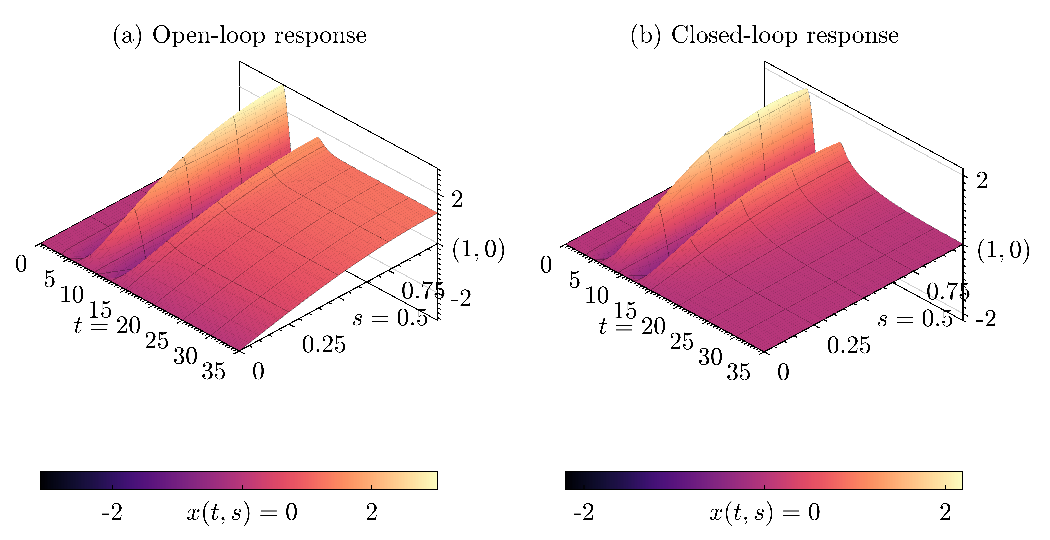
\includegraphics[width=.495\textwidth]{Figures/example3_state.pdf}
 \caption{Open- and closed-loop state responses for the nonlinear
 reaction--diffusion equation (left pair) and the damped wave equation
 (right pair). Disturbed by $w_{\mrm p}(t)=8\cos(t)\mathbf 1_{[\pi,4\pi]}(t)$.}
 \label{fig:sector-pde-states}
\end{figure*}
\begin{figure}[t]
 \centering
 
\includegraphics[width=.495\columnwidth]{Figures/example2_effort.pdf}\hfill
 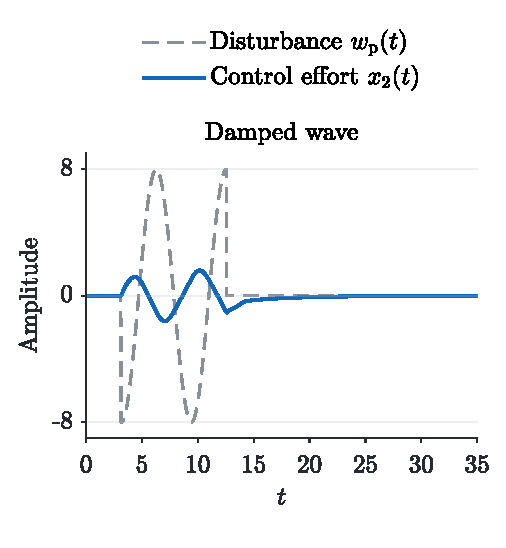
\includegraphics[width=.495\columnwidth]{Figures/example3_effort.pdf}
 \caption{Disturbance and control effort for the reaction--diffusion
 equation (left) and damped wave equation (right).}
 \label{fig:sector-pde-effort}
\end{figure}


